\section{Results} \label{sresults}

\subsection{Parallelism in Cilk programs}

\begin{table}
\small
\begin{tabular}{ | l | l | l | }
\hline
Program & Description & Parameters \\
\hline
cholesky & Matrix decomposition & \texttt{size=256}, \texttt{nonzeros=1000} \\
cilksort & Merge sort & \texttt{size=100000} \\
fft & Fourier transform & \texttt{size=512*512} \\
fib & Na\"ive Fibonacci calculation & \texttt{n=30} \\
heat & Differential equation solver & \texttt{nx=ny=512}, \texttt{nt=1} \\ 
lu & Matrix decomposition & \texttt{n=256} \\
magic & Magic squares search & \texttt{n=4} \\
matmul & Matrix multiplication & \texttt{n=128} \\
plu & Matrix decomposition & \texttt{n=128} \\
strassen & Matrix multiplication & \texttt{n=512} \\
\hline
\end{tabular}
\caption{Description and parameters for Cilk 5.4.6 examples used}
\label{cilk-ex}
\end{table}

We begin by presenting the results of analysing example Cilk programs packaged with the 5.4.6 release of Cilk, as described in Table~\ref{cilk-ex}\footnote{We have omitted programs that use the \texttt{inlet}, \texttt{abort} and \texttt{SYNCHED} keywords, as their translation into ordinary C is not straightforward.}.
As examples packaged with a parallel programming environment, these are programs known to have lots of task-level parallelism.
We ran the original programs in Cilk a number of times to obtain a figure for average parallelism as calculated by the Cilk infrastructure.
We then translated these programs into semantically equivalent programs in ordinary C simply by stripping the Cilk keywords\footnote{Namely, \texttt{cilk}, \texttt{spawn} and \texttt{sync}.}.
These \emph{serial elisions} of the original programs are then analysed with our extension of Embla under a number of different models.

\begin{figure}
 \centering
 \includegraphics[width=3in]{cilk-run}
 \caption{Parallelism of Cilk programs as calculated by Cilk and Embla}
 \label{cilk-run}
\end{figure}

Figure~\ref{cilk-run} compares the parallelism found by Cilk (averaged over 60 runs) to that found by our extension of Embla on their serial elisions.
Our baseline model for this comparison uses agreegated data dependences and control dependences, and considers only function-call-level parallelism without loop parallelization or spawn hoisting---the closest model to the one used in Cilk.
We can observe that our tool is able to find all of the task-level parallelism in most of the original Cilk programs.
The only exceptions are fib and magic, the Cilk parallelism for which appears to vary greatly.
The reason our tool does not find much parallelism in magic compared to the Cilk run is because the Cilk program uses an associative reduction variable in a loop which sums over the results of each iteration, in the form \texttt{for (...) count += spawn(...);}.
Our tool currently cannot recognize associative reduction variables, and therefore cannot discover such parallelism.

\begin{figure}
  \begin{center}
  \scriptsize
  \input{cilksort.depgraph}
  \end{center}
  \nocaptionrule \caption{An extract from cilksort and its corresponding relevant dependences}
  \label{cilksort-depgraph}
\end{figure}

Using aggregated dependences discovered by our tool it is easy to re-insert Cilk keywords into the program to materialize the parallelism discovered.
As an example, Figure~\ref{cilksort-depgraph} shows the aggregated dependences that our tool found for an extract from the cilksort program.
Observe that simply by inserting \texttt{spawn}s in front ot function calls, and \texttt{sync}s before the first line that depends on previously spawned tasks, we arrive at the original program.

\begin{figure}
  \begin{center}
  \small
  \begin{SubFloat}{\label{cilk-sync:without}Original program, showing dependences and best possible parallelization with universal \texttt{sync}s}
    \begin{minipage}{3in}
      \input{lu.depgraph}
    \end{minipage}%
  \end{SubFloat}%
\\
  \begin{SubFloat}{\label{cilk-sync:with}Best possible parallelization if individual \texttt{sync}s were allowed}
    \begin{minipage}{3in}
      \begin{verbatim}
future1 = spawn schur(M00, V00, W00, hnb);
future2 = spawn schur(M01, V00, W01, hnb);
future3 = spawn schur(M10, V10, W00, hnb);
future4 = spawn schur(M11, V10, W01, hnb);

sync future1;
spawn schur(M00, V01, W10, hnb);
sync future2;
spawn schur(M01, V01, W11, hnb);
sync future3;
spawn schur(M10, V11, W10, hnb);
sync future4;
spawn schur(M11, V11, W11, hnb);
      \end{verbatim}
    \end{minipage}%
  \end{SubFloat}%
  \end{center}
  \caption{An example of the greater parallelism caused by individual \texttt{sync}s in an extract from lu.}
  \label{cilk-sync}
\end{figure}


In fact, for a few examples our tool can discover more parallelism than explicitly specified in the original Cilk program.
We found functions called sequentially in cholesky, heat and strassen that could have been spawned.
In addition, we also found C library function calls in heat, lu and plu that cannot be spawned directly in Cilk (as library functions are not defined as spawnable) but can be spawned with the addition of simple wrappers.
The greater parallelism found in cholesky, lu and plu can also be partly attributed to a restriction in Cilk that \texttt{sync}s must join on all tasks spawned rather than any individual task.
If tasks could be synchronized on individually, as illustrated in Figure~\ref{cilk-sync} then greater parallelism may be found.

We now look more closely at the various models used to examine whether they affect potential parallelism in these programs.

\subsubsection{Data dependences}

\begin{figure}
 \centering
 \includegraphics[width=3in]{cilk-data}
 \caption{Parallelism of Cilk programs with aggregated and exact data dependences}
 \label{cilk-data}
\end{figure}

Figure~\ref{cilk-data} shows the potential parallelism of the serial elisions of our Cilk examples with aggregated and exact data dependences.
In all programs but lu we see that the difference between the two models is negligible,
This suggests that for most programs most of the potential parallelism is achievable by adding parallel constructs at the source level---runtime techniques such as thread-level speculation would give few performance benefits.

\subsubsection{Control dependences}

\begin{figure}
 \centering
 \includegraphics[width=3in]{cilk-ctl}
 \caption{Parallelism of Cilk programs with and without control dependences}
 \label{cilk-ctl}
\end{figure}

The effects of control speculation are shown in Figure~\ref{cilk-ctl}, which compares the parallelism when control dependences are considered to that when they are ignored.
For these programs we can see that control speculation does not have any effect on available parallelism.
One possible reason for this is that most of these programs are stream-processing-like, with few branches that depend on the data input.
More irregular programs may see greater improvements with control speculation.

\subsubsection{Granularity}

\begin{figure}
 \centering
 \includegraphics[width=3in]{cilk-gran}
 \caption{Parallelism of Cilk programs with different levels of granularity}
 \label{cilk-gran}
\end{figure}

The amount of line-level parallelism in these programs is compared to the amount of task-level parallelism in Figure~\ref{cilk-gran}.
We can see that for most of these programs the amount of line-level parallelism is around twice or more the amount of function-call-level parallelism.
Most of this difference is due to simple statements that perform arithmetic operations inside a function call or loop that can run in parallel.
Each of these operations takes a small number of cycles, which means that it is not viable for each of these to be spawned.
Nevertheless, operations may be grouped and extracted into tasks that are sufficiently large to see performance gains.
We also note that some of this parallelism may well be realized already in existing superscalar or VLIW processors.

\subsubsection{Loops}

\begin{figure}
 \centering
 \includegraphics[width=3in]{cilk-loop}
 \caption{Parallelism of Cilk programs with and without spawning loop iterations}
 \label{cilk-loop}
\end{figure}

Looking at Figure~\ref{cilk-loop}, which compares the potential parallelism of Cilk programs with and without spawning loop iterations, we can see that the use of parallel for-loops benefit most of the programs considered here.
This is most remarkable in matmul, where there is a 64-fold gain in parallelism when for loops are parallelized.
We deduce from this that the use of parallel for-loops is an excellent tool for expressing task-level parallelism, in addition to function calls.
Indeed, this validates the inclusion of parallel for-loops in Cilk++, the commercialized version of Cilk.
Our extension of Embla not only finds the amount of loop-level parallelism in a program, but can be used to easily identify candidate loops for parallelization.
It can simply be done by searching through the dependences output by our tool for dependences between iterations of the loop concerned.
If there are no such dependences, then the loop can be parallelized.

\subsubsection{Spawn hoisting}

\begin{figure}
 \centering
 \includegraphics[width=3in]{cilk-hoist}
 \caption{Parallelism of Cilk programs with and without spawn hoisting}
 \label{cilk-hoist}
\end{figure}

Figure~\ref{cilk-hoist} shows little effect of spawn hoisting on the amount of potential parallelism in the Cilk examples.
This suggests that most function calls are already spawned at the earliest possible point in the program, and there is little further hoisting possible.

\subsection{Parallelism in various benchmarks}

\begin{figure*}
 \centering
 \subfloat[SPEC CPU 2000 integer benchmarks]{
   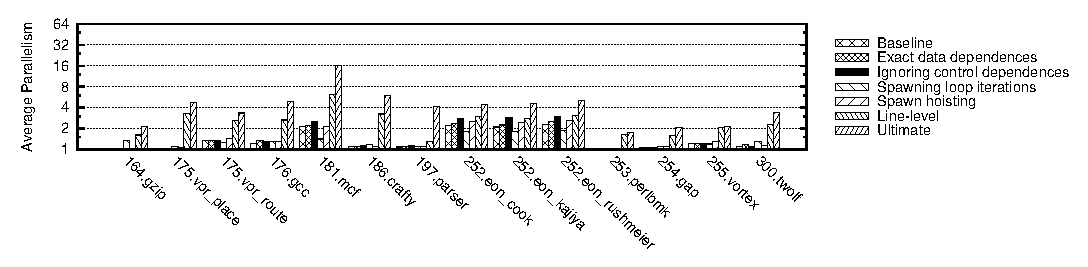
\includegraphics[width=6.5in]{spec}
 }
 \subfloat[SPEC CPU 2000 floating point benchmarks]{
   \includegraphics[width=6.5in]{specfp}
 }
 \subfloat[miBench]{
   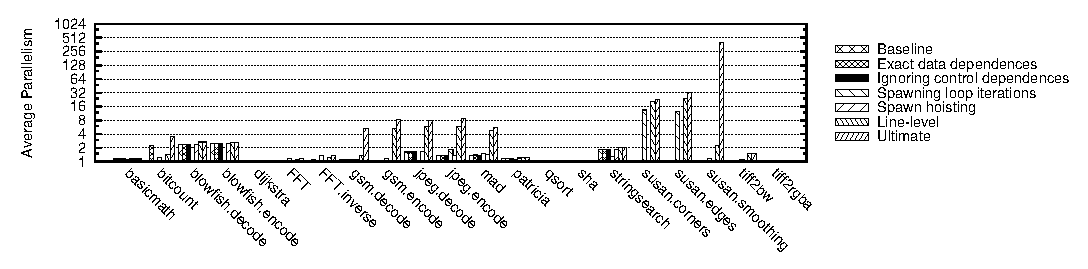
\includegraphics[width=6.5in]{mb}
 }

\caption{Parallelism of three benchmark suites under various models}
\label{benchmarks}
\end{figure*}

We also ran the same analysis using our tool on some of benchmark programs in the SPEC CPU 2000 (with the MinneSPEC reduced data input set \cite{KleinOsowski02minnespec}) and miBench suites, the results of which are displayed in Figure~\ref{benchmarks}.
As before, the baseline model uses agregated data dependences and control dependences, and considers only function-call-level parallelism without loop parallelization or spawn hoisting.
Each of the other models differs from the baseline by one parameter described in Section~\ref{smethod}, except for Ultimate, which considers line-level parallelism by using exact data dependences, ignoring control dependences and hoisting spawns.
In general, we see that few benchmarks exhibit the level of parallelism seen in the Cilk examples.
In fact, none of these benchmarks exhibit parallelism of over 3 under the baseline model.

There are, however, some benchmarks with a significant amount of loop-level parallelism.
One of them is the miBench benchmark SUSAN, a program that performs image smoothing, corner detection and edge detection on an image, and is data-parallel---the same computation is performed on each pixel in the image and the results for each pixel are independent of each other.
This is reflected in our results, which show that both susan.corners and susan.edges have potential parallelism of over 12 when loop iterations are spawned.
The same would have been true for susan.smoothing had it not had an associative reduction variable in the loop, which as mentioned our tool currently cannot recognize.

We note also that for some programs, e.g.\ eon, spawning loop iterations actually results in a \emph{lower} level of parallelism.
This is because that while spawning loop iterations allows us to exploit DOALL parallelism, where loop iterations are completely independent from each other and can be executed in parallel, it precludes DOACROSS parallelism or software pipelining, where there are cross-iteration dependences but loop iterations can still partially overlap.
The balance between DOALL and DOACROSS loops would therefore determine whether parallelism rises or falls compared to the baseline.

\subsection{Discussion}

Our results suggest that while the example programs from Cilk have lots of inherent task-level parallelism, most general-purpose programs tend to have little and cannot be transformed into highly concurrent programs simply by spawning existing function calls and loops.
Nevertheless, our extension of Embla can output the critical path of each function call, allowing us to examine the bottlenecks that prevent greater parallelism from being realized.
Having examined several programs in more detail, we now present some of the reasons why they exhibit such low levels of parallelism, and suggest what can be done to increase their potential.

\subsubsection{sha}

\begin{figure}
  \begin{center}
    \scriptsize
    \begin{SubFloat}{\label{sha-bottleneck:critpath}Critical path for a call to the \texttt{sha\_stream} function, produced by our tool}
      \begin{minipage}{3in}
        \begin{verbatim}
!sha_driver.c:24(sha.c)=16139892:
200(3460), 198(26614), 198(423934), 198(423934),
198(423934), 198(423934), 198(423934), 198(423934),
198(423934), 198(423934), 198(423934), 198(423934),
198(423934), 198(423934), 198(423934), 198(423934),
198(423934), 198(423934), 198(423934), 198(423934),
198(423934), 198(423934), 198(423934), 198(423934),
198(423934), 198(423934), 198(423934), 198(423934),
198(423934), 198(423934), 198(423934), 198(423934),
198(423934), 198(423934), 198(423934), 198(423934),
198(423934), 198(423934), 198(423934), 198(423934),
197(326)
        \end{verbatim}
      \end{minipage}
    \end{SubFloat}
\\
    \begin{SubFloat}{\label{sha-bottleneck:source}Source for \texttt{sha\_stream} function in \texttt{sha.c}}
      \begin{minipage}{3in}
        \begin{verbatim}
191  void sha_stream(SHA_INFO *sha_info, FILE *fin)
192  {
193      int i;
194      BYTE data[BLOCK_SIZE];
195
196      sha_init(sha_info);
197      while ((i = fread(data, 1, BLOCK_SIZE, fin)) > 0) {
198          sha_update(sha_info, data, i);
199      }
200      sha_final(sha_info);
201  }
        \end{verbatim}
      \end{minipage}
    \end{SubFloat}
  \end{center}
  \caption{Critical Path Analysis of SHA}
  \label{sha-bottleneck}
\end{figure}

SHA, or Secure Hash Algorithm, is a program that computes a 160-bit hash value from the contents of an input file.
Figure~\ref{sha-bottleneck} illustrates part of our analysis into the reason for the lack of inherent parallelism there.
Under a model with line-level parallelism, our tool has reported a critical path of length 16150120 instructions out of a total of 21968394 instructions, resulting in a parallelism of 1.36.
From Figure~\ref{sha-bottleneck:critpath}, we see that most of the critical path (16139892 instructions) is due to a function call on line 24 in the file \texttt{sha\_driver.c}.
We also see that the critical path consists mainly of dependences between instantiations of line 198 in \texttt{sha.c}, most of which have a cost of 423934 instructions.
These correspond to calls to \texttt{sha\_update} in the program source (Figure~\ref{sha-bottleneck:source}).

Further examination of \texttt{sha\_update} reveals that the function takes the existing hash value (the \emph{digest}) and derives a new hash value which replaces it.
Consequently, each call to this function must depend on the last as it requires the digest computed by the last call.
In order to increase the amount of inherent parallelism, an alternative algorithm can be used, e.g.\ by dividing the file into blocks and computing digests for each block, which are then combined into one final digest.

\subsubsection{186.crafty}

Crafty is a chess-playing program that uses a Minimax-like algorithm to find the best move through searching a game tree.
In theory game tree searching is an easily parallelizable activity, as demonstrated by the success of multi-threaded chess-playing programs \cite{Dailey01usingcilk}.
However, our tool does not find plenty of parallelism in Crafty for a number of reasons.
Firstly, Crafty uses one global chessboard, which is updated when a move is considered and then reverted afterwards, creating a chain of data dependences that linearize the search.
Furthermore, various pruning techniques used mean that later searches are influenced by the results of earlier ones.
This shows that algorithmic changes are required before such a program can be parallelized.

\subsubsection{164.gzip}

Gzip is a file compression program.
It works by traversing the input file sequentially, looking for recurrences of substrings that have been seen before.
As such it is easy to see that the program cannot process the later parts of the file before the earlier parts have been processed---this results in little task-level parallelism.
One could imagine changing the algorithm such that a file is divided into blocks that are compressed independently, resulting in greater parallelism at the cost of a larger output file.

\subsubsection{Input/output}

We find that input/output forms a large part of several benchmarks.
In dijkstra, for example, a tenth of the program's sequential execution time is taken up by calls to \texttt{scanf}.
In FFT (miBench), printing the results takes up around 80\% of processing time.
If we assume that input/output is unparallelizable, Amdahl's law would mean that the maximum speed-up, even if we were able to parallelize the rest of the program perfectly, would still be low.
This suggests that for some of the benchmarks examined, a parallel implementation of input/output would be very useful.

\subsubsection{Getting more parallelism from loops}

\begin{figure}
  \centering
  \begin{SubFloat}{\label{dnc:orig}Original program}
    \begin{minipage}{3in}
      \begin{verbatim}
for (j = n = 0, seed = rand();
     j < iterations;
     j++, seed += 13) {
  int r = pBitCntFunc[i](seed);
  n += r;
}
      \end{verbatim}
    \end{minipage}%
  \end{SubFloat}%
\\
  \begin{SubFloat}{\label{dnc:trans}Transformed program}
    \begin{minipage}{3in}
      \begin{verbatim}
int dc_bitcnts(int start, int n_itrs, int i) {
  if (n_itrs <= 0) return 0;
  if (n_itrs == 1) return pBitCntFunc[i](start);
  else {
    int x,y;
    int half_itrs = n_itrs / 2;
    x = dc_bitcnts(start, half_itrs, i);
    y = dc_bitcnts(start+(half_itrs*13),
          n_itrs - half_itrs, i);
    return x+y;
  }
}

n = dc_bitcnts(seed, iterations, i);
      \end{verbatim}
    \end{minipage}%
  \end{SubFloat}%
  \caption{Tranformation of a loop in the bitcount program using divide and conquer.}
  \label{dnc}
\end{figure}

Despite the relatively low figures of parallelism, there are some simple ways of modifying a program to unlock greater parallelism, one of which we present here.
Figure~\ref{dnc} shows a transformation applied to a (slightly adapted) loop in the bitcount benchmark.
In the original program, calls to \texttt{pBitCntFunc[i]} are pure and can be run in parallel with each other.
However, there is a dependence between increments of the induction variables, \texttt{j} and \texttt{seed}, and between additions to the accumulator \texttt{n}, producing two long chains of data dependences.
Nevertheless, by recognising that \texttt{n} is a reduction variable we can transform the loop into recursive calls using a divde-and-conquer strategy.
The lengths of the dependence chains on the induction and reduction variables become logarithmic on the number of iterations instead of linear, and consequently the critical path found by our tool is a tenth of that in the original program, despite the overheads of extra function calls.
This shows that simple transformations can sometimes be sufficient to increase the amount of potential parallelism in certain programs.
In fact, we note that Cilk++, the commercialized version of Cilk, indeed uses a divide-and-conquer strategy for its parallel for-loops, a decision which is justified by our example.

